\chapter{Infinite Series}
\label{ch:series}

\section{Series, Partial Sums, and the Cauchy Criterion}

An infinite sum is never formed by adding infinitely many terms at once.
Its mathematical meaning is the limit of finite partial sums, so all
questions about series begin with the sequence theory already developed.

\begin{definition}[Series]
Let $(a_n)$ be a real sequence. Its $N$th \textbf{partial sum} is
\[
s_N=\sum_{n=1}^{N}a_n.
\]
The \textbf{series} with terms $(a_n)$ is denoted by
\[
\sum_{n=1}^{\infty}a_n.
\]
It \textbf{converges} when $(s_N)$ converges; its sum is then
\[
\sum_{n=1}^{\infty}a_n=\lim_{N\to\infty}s_N.
\]
\end{definition}

\begin{theorem}[Cauchy criterion for series]
\label{thm:series-cauchy}
The series
\[
\sum_{n=1}^{\infty}a_n
\]
converges if and only if, for every $\eps>0$, there is $N\in\N$ such that
\[
m>n\geq N
\quad\Longrightarrow\quad
\abs{\sum_{k=n+1}^{m}a_k}<\eps.
\]
\end{theorem}
\begin{proof}
For $m>n$,
\[
s_m-s_n=\sum_{k=n+1}^{m}a_k.
\]
Thus the stated condition says exactly that the partial sums are Cauchy. Apply \cref{thm:cauchy-criterion}.
\end{proof}

\begin{proposition}[Finite changes and telescoping]
\label{prop:finite-changes-telescoping}
Changing finitely many terms of a series does not affect convergence. If
\[
a_n=b_n-b_{n+1},
\]
then
\[
\sum_{n=1}^{N}a_n=b_1-b_{N+1}.
\]
Consequently, this telescoping series converges if and only if $(b_n)$ converges, and its sum is
\[
b_1-\lim_{n\to\infty}b_n.
\]
\end{proposition}
\begin{proof}
Partial sums after a finite change differ by a constant from some point onward. The displayed finite identity follows by cancellation; its limit proves the last assertion.
\end{proof}

\begin{proposition}[Necessary condition]
\label{prop:series-terms-zero}
If a series converges, then its terms tend to zero.
\end{proposition}
\begin{proof}
If $s_N\to s$, then
\[
a_N=s_N-s_{N-1}
\qquad(N\geq2).
\]
The algebra of limits gives $a_N\to0$.
\end{proof}

\begin{remark}[Preliminary strategy for choosing a test]
Before trying a sophisticated theorem, check the necessary condition
$a_n\to0$; failure settles divergence, although success proves nothing by
itself.  Next look for exact geometric or telescoping structure.  For
nonnegative terms, compare with an already understood benchmark.  Factorials
and exponentials often favor the Ratio Test, while expressions raised to the
$n$th power often favor the Root Test.  Alternating signs suggest checking
absolute convergence first and then the Alternating-Series Test.  An
inconclusive test is information about the test, not a verdict about the
series.
\end{remark}

\section{Nonnegative Series and Comparison}

When terms are nonnegative, partial sums can only increase.  This lets order
and completeness convert estimates by simpler benchmark series into decisive
convergence tests.

\begin{theorem}[Comparison test]
\label{thm:comparison-test}
Let
\[
0\leq a_n\leq b_n
\qquad(n\in\N).
\]
If
\[
\sum_{n=1}^{\infty}b_n
\]
converges, then
\[
\sum_{n=1}^{\infty}a_n
\]
converges. If the latter series diverges, then the former diverges.
\end{theorem}
\begin{proof}
The partial sums of $(a_n)$ are increasing and bounded above by the sum of the series with terms $b_n$. Apply \cref{thm:monotone-convergence}. The second statement is the contrapositive.
\end{proof}

\begin{theorem}[Limit comparison test]
\label{thm:limit-comparison}
Let $a_n,b_n>0$ eventually, and suppose
\[
\lim_{n\to\infty}\frac{a_n}{b_n}=L
\]
with
\[
0<L<\infty.
\]
Then the series with terms $a_n$ converges if and only if the series with terms $b_n$ converges.
\end{theorem}
\begin{proof}
Choose $N_0$ from which both sequences are positive, and $N_1$ from
the limit definition with tolerance $L/2$. For every
$n\geq N=\max\{N_0,N_1\}$,
\[
\left|\frac{a_n}{b_n}-L\right|<\frac L2,
\qquad \frac L2<\frac{a_n}{b_n}<\frac{3L}{2}.
\]
Multiplication by $b_n>0$ gives
\[
\frac L2b_n<a_n<\frac{3L}{2}b_n.
\]
The upper bound compares $\sum a_n$ with a convergent multiple of
$\sum b_n$; the lower bound can be rewritten $b_n<(2/L)a_n$ for
the reverse implication. Apply \cref{thm:comparison-test} in both
directions and \cref{prop:finite-changes-telescoping} to discard the
finite initial segment. The particular constants do not matter; the tail
is controlled by fixed positive multiples.
\end{proof}

\begin{theorem}[Geometric series]
\label{thm:geometric-series}
For $r\in\R$, the series with terms $r^n$, beginning at $n=0$, converges if and only if
\[
\abs r<1.
\]
In that case,
\[
\sum_{n=0}^{\infty}r^n=\frac{1}{1-r}.
\]
\end{theorem}
\begin{proof}
For $r\ne1$,
\[
\sum_{n=0}^{N}r^n=\frac{1-r^{N+1}}{1-r}.
\]
If $r=0$, the conclusion is immediate. If $0<r<1$, write $r=1/(1+h)$ with $h>0$. Bernoulli's inequality gives
\[
(1+h)^N\geq1+Nh,
\]
so
\[
0\leq r^N\leq\frac{1}{1+Nh}\longrightarrow0.
\]
The same conclusion holds whenever $\abs r<1$, because
\[
\abs{r^N}=\abs r^N.
\]
Taking limits proves the formula. If $\abs r\geq1$, the terms do not tend to zero, so \cref{prop:series-terms-zero} proves divergence.
\end{proof}

Multiplying by an initial coefficient $a$ gives the usual general form:
\[
\sum_{k=0}^{\infty}ar^k=\frac{a}{1-r}\qquad(|r|<1).
\]
Here $a$ is the first term and $r$ the common ratio. If $a=0$, the series
is zero for every $r$; the necessity of $|r|<1$ applies when $a\ne0$.

The condensation test groups terms into blocks of doubling length:
\[
\underbrace{b_1}_{1\text{ term}},\quad
\underbrace{b_2+b_3}_{2\text{ terms}},\quad
\underbrace{b_4+\cdots+b_7}_{4\text{ terms}},\quad
\underbrace{b_8+\cdots+b_{15}}_{8\text{ terms}}.
\]
On the $k$th block all $2^k$ terms lie between the values at its ends.
Comparing one block at a time gives the inequalities in the proof; it
does not replace every term by an asymptotic guess.
\begin{theorem}[Cauchy condensation test]
\label{thm:cauchy-condensation}
Let $(b_n)$ be a nonincreasing sequence of nonnegative real numbers. Then
\[
\sum_{n=1}^{\infty}b_n
\]
converges if and only if
\[
\sum_{k=0}^{\infty}2^k b_{2^k}
\]
converges.
\end{theorem}
\begin{proof}
For every $k\geq0$,
\[
2^k b_{2^{k+1}}
\leq
\sum_{n=2^k}^{2^{k+1}-1}b_n
\leq
2^k b_{2^k}.
\]
Summing the right inequalities proves that convergence of the condensed series implies convergence of the original series. Summing the left inequalities gives
\[
\frac12\sum_{k=1}^{m+1}2^k b_{2^k}
\leq
\sum_{n=1}^{2^{m+1}-1}b_n.
\]
Hence boundedness of the original partial sums implies boundedness of the condensed partial sums. Both series have nonnegative terms, so monotone convergence completes the proof.
\end{proof}

\begin{example}[Recognizing a finite cancellation]
For $a_n=1/(n(n+1))$, write $a_n=1/n-1/(n+1)$.
The $N$th partial sum is $1-1/(N+1)$, so the sum is $1$.
The finite identity must come before passage to an infinite sum.
For comparison, $1/(n(n+1)+1)\leq1/(n(n+1))$ for $n\geq1$,
so its series converges without an exact formula for its sum.
\end{example}

\begin{example}[Accumulating repeated contributions]
A sequence of corrections adds $1/2$ millimetre initially, and each
subsequent correction adds half the preceding amount. After $N$
corrections the total is $s_N=\sum_{n=1}^N2^{-n}=1-2^{-N}$
millimetres. The geometric-series theorem proves a limiting total of
$1$ millimetre, and the unperformed corrections total $2^{-N}$
millimetres. Thus $N=10$ gives an error below $1/1000$ millimetre.
Writing an infinite sum only proposes the accumulated quantity;
convergence proves that the proposed total is finite.
\end{example}

\section{Absolute Convergence and Products}

Signs permit cancellation, which is useful but dangerous: a series can look
small only because large positive and negative tails offset each other.
Absolute convergence rules out that instability and will justify changing
orders and multiplying series.

\begin{definition}[Absolute and conditional convergence]
A series with real terms $a_n$ \textbf{converges absolutely} if
\[
\sum_{n=1}^{\infty}\abs{a_n}
\]
converges. It \textbf{converges conditionally} if it converges but does not converge absolutely.
\end{definition}

Absolute convergence controls the total size of the terms and will justify rearrangement. Conditional convergence is weaker, so changing the order of its terms requires separate care.

\begin{theorem}[Absolute convergence test]
\label{thm:absolute-convergence}
Absolute convergence implies convergence.
\end{theorem}
\begin{proof}
For $m>n$,
\[
\abs{\sum_{k=n+1}^{m}a_k}
\leq
\sum_{k=n+1}^{m}\abs{a_k}.
\]
The Cauchy criterion for the absolute-value series and \cref{thm:series-cauchy} show that the original partial sums are Cauchy.
\end{proof}

\begin{theorem}[Weierstrass M-test]
\label{thm:weierstrass-m-test}
Let $f_n:D\to\R$ be functions, and suppose that there are numbers $M_n\geq0$
such that
\[
\abs{f_n(x)}\leq M_n
\qquad(x\in D, n\in\N).
\]
If
\[
\sum_{n=1}^{\infty}M_n
\]
converges, then
\[
\sum_{n=1}^{\infty}f_n
\]
converges uniformly and absolutely on $D$.
\end{theorem}
\begin{proof}
For $q\geq p$,
\[
\abs{\sum_{n=p}^{q}f_n(x)}
\leq\sum_{n=p}^{q}\abs{f_n(x)}
\leq\sum_{n=p}^{q}M_n.
\]
Given $\eps>0$, choose $N$ from the numerical Cauchy criterion so
that $\sum_{n=p}^q M_n<\eps$ whenever $q\geq p\geq N$.
The final bound is independent of $x$ and works for all these indices.  The uniform Cauchy
criterion of Chapter~\ref{ch:function-sequences} proves uniform convergence.
The same estimate applied to $\abs{f_n}$ proves absolute convergence at every
point.
\end{proof}

\begin{example}[A uniform majorant]
On $[-1,1]$,
\[
\abs{\frac{x^n}{2^n}}\leq\frac1{2^n}.
\]
Since $\sum_{n=1}^{\infty}2^{-n}$ converges, the M-test shows that
\[
\sum_{n=1}^{\infty}\frac{x^n}{2^n}
\]
converges uniformly and absolutely on $[-1,1]$.
\end{example}

\begin{theorem}[Rearrangement of an absolutely convergent series]
\label{thm:absolute-rearrangement}
Let
\[
\sum_{n=1}^{\infty}a_n
\]
converge absolutely, and let $(a_{\sigma(n)})$ be a rearrangement, where $\sigma:\N\to\N$ is a bijection. Then the rearranged series converges absolutely and has the same sum.
\end{theorem}
\begin{proof}
\textbf{Strategy.} Wait until every important early term has appeared;
all remaining terms belong to a small absolute tail.
Put $S=\sum_{n=1}^\infty a_n$ and $A=\sum_{n=1}^\infty|a_n|$.
Every rearranged absolute partial sum is at most $A$, so monotone
convergence proves absolute convergence of the rearranged series.
Given $\eps>0$, choose $N$ with $\sum_{r>N}|a_r|<\eps/2$.
Let $M=\max\{\sigma^{-1}(1),\ldots,\sigma^{-1}(N)\}$.
For every $m\geq M$, $I_m=\{\sigma(1),\ldots,\sigma(m)\}$
contains $\{1,\ldots,N\}$. Hence
\[
\left|\sum_{j=1}^m a_{\sigma(j)}-S\right|
\leq\left|\sum_{r\in I_m\setminus\{1,\ldots,N\}}a_r\right|
+\left|\sum_{r=1}^N a_r-S\right|
\leq 2\sum_{r>N}|a_r|<\eps.
\]
Thus the sums agree.
\end{proof}

A product of finite partial sums sums over a rectangle of index pairs
$(j,k)$. A Cauchy product instead collects pairs along diagonals $j+k=n$;
its partial sums fill a triangle. Absolute convergence controls the terms
in the difference of those two shapes.
\begin{center}
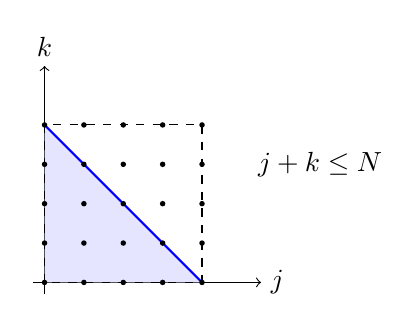
\begin{tikzpicture}[scale=.5]
\draw[->] (-.3,0)--(5.5,0) node[right] {$j$};
\draw[->] (0,-.3)--(0,5.5) node[above] {$k$};
\fill[blue!10] (0,0)--(4,0)--(0,4)--cycle;
\draw[blue,thick] (0,4)--(4,0); \draw[dashed] (0,0) rectangle (4,4);
\foreach \x in {0,1,2,3,4}{\foreach \y in {0,1,2,3,4}{\fill (\x,\y) circle (.07);}}
\node at (7,3) {$j+k\leq N$};
\end{tikzpicture}
\end{center}
\begin{theorem}[Cauchy product]
\label{thm:cauchy-product}
Suppose that
\[
\sum_{n=0}^{\infty}a_n
\quad\hbox{and}\quad
\sum_{n=0}^{\infty}b_n
\]
converge absolutely. Define
\[
c_n=\sum_{k=0}^{n}a_kb_{n-k}.
\]
Then
\[
\sum_{n=0}^{\infty}c_n
\]
converges absolutely and
\[
\left(\sum_{n=0}^{\infty}a_n\right)
\left(\sum_{n=0}^{\infty}b_n\right)
=\sum_{n=0}^{\infty}c_n.
\]
\end{theorem}
\begin{proof}
The partial sums of
\[
\sum_{n=0}^{\infty}\abs{c_n}
\]
are bounded by the product of the two absolute sums, because
\[
\sum_{n=0}^{N}\abs{c_n}
\leq
\sum_{\substack{j,k\geq0\\j+k\leq N}}\abs{a_j}\abs{b_k}.
\]
Thus the Cauchy product converges absolutely. Let $\eps>0$. Choose $K$ so large that
\[
\left(\sum_{j=K+1}^{\infty}\abs{a_j}\right)
\left(\sum_{k=0}^{\infty}\abs{b_k}\right)
+
\left(\sum_{j=0}^{\infty}\abs{a_j}\right)
\left(\sum_{k=K+1}^{\infty}\abs{b_k}\right)
<\eps.
\]
For $N\geq2K$, every pair $(j,k)$ with
\[
0\leq j,k\leq N,\qquad j+k>N
\]
has either $j>K$ or $k>K$. Distributivity of finite sums gives the exact identity
\[
\left(\sum_{j=0}^N a_j\right)\left(\sum_{k=0}^N b_k\right)
-\sum_{n=0}^N c_n
=\sum_{\substack{0\leq j,k\leq N\\j+k>N}}a_jb_k.
\]
The absolute value of the right side is bounded by
\[
\left(\sum_{j>K}|a_j|\right)\left(\sum_{k\geq0}|b_k|\right)
+\left(\sum_{j\geq0}|a_j|\right)\left(\sum_{k>K}|b_k|\right)<\eps.
\]
The finite product tends to the product of the two original sums. Its
difference from the Cauchy partial sum tends to zero, proving the formula.
No infinite double series has been rearranged in this argument.
\end{proof}

\section{Ratio, Root, and Alternating Tests}

Many series are best compared not term by term with a fixed model, but by
examining how consecutive terms or their roots behave.  The following tests
make that asymptotic comparison precise.

\paragraph{Rational powers are already available.}
Recall from \cref{def:rational-powers,lem:rational-power-laws} in
Chapter~\ref{ch:continuity} that positive rational powers are well defined,
independent of the fraction representing the exponent, and satisfy the usual
exponent and order laws. We now use that established algebraic language in
the Root Test and the rational (p)-series theorem; constructing it no longer
interrupts the series narrative.

\begin{remark}[Informal calculus preview: the Integral Test]
\label{rem:integral-test-preview}
This paragraph recalls familiar calculus without using it as a proof
prerequisite. Improper integrals have not yet been formally defined.
In this preview only, the familiar notation for arbitrary real powers
is allowed; Chapter~\ref{ch:differentiation} constructs those powers.
The familiar rule is that $\sum_{n=1}^\infty1/n^p$ converges exactly
when $p>1$. The Integral Test says that for a positive continuous
decreasing $f$ on $[1,\infty)$, $\sum f(n)$ and
$\int_1^\infty f(x)\,\dd x$ have the same convergence behavior.

Recall the calculus procedure: truncate, evaluate the proper integral,
then take the endpoint limit. For example,
\[
\int_1^b\frac{\dd x}{x^2}=1-\frac1b\to1,\qquad
\int_1^b\frac{\dd x}{\sqrt{x}}=2(\sqrt b-1)\to+\infty.
\]
The preview predicts convergence of $\sum1/n^2$ and divergence of
$\sum1/\sqrt n$. At a singular left endpoint use
$\lim_{c\to a^+}\int_c^b f$; at a singular right endpoint use
$\lim_{c\to b^-}\int_a^c f$. Different improper pieces must converge
separately: cancellation of divergent pieces is not allowed.
Chapter~\ref{ch:riemann}, especially \cref{thm:integral-test}, will
define these limits and prove the test. The next theorem independently
proves the rational-$p$ rule by condensation, with no integration.
\end{remark}

\begin{theorem}[Rational $p$-series test]
\label{thm:rational-p-series-test}
Let
\[
p\in\Q.
\]
Then
\[
\sum_{n=1}^{\infty}\frac{1}{n^p}
\]
converges if and only if
\[
p>1.
\]
\end{theorem}
\begin{proof}
Suppose first that
\[
p>0.
\]
By \cref{lem:rational-power-laws}, the sequence
\[
b_n=n^{-p}
\]
is nonincreasing. The Cauchy Condensation Test gives convergence precisely when
\[
\sum_{k=0}^{\infty}2^k(2^k)^{-p}
=\sum_{k=0}^{\infty}2^{k(1-p)}
\]
converges. This is a geometric series with positive ratio
\[
2^{1-p};
\]
by the order statement in \cref{lem:rational-power-laws}, that ratio is less than $1$ exactly when
\[
p>1.
\]
If
\[
p\leq0,
\]
then
\[
n^{-p}\geq1
\qquad(n\in\N),
\]
so the terms do not tend to zero. The necessary condition in \cref{prop:series-terms-zero} proves divergence.
\end{proof}




\begin{example}[Choosing a benchmark]
For $a_n=(3n+1)/(n^3+2)$, compare with $b_n=1/n^2$.
Then $a_n/b_n=(3+1/n)/(1+2/n^3)\to3$, so limit comparison and
the rational $p$-series theorem give convergence. For
$c_n=1/\sqrt{n^2+n}$, comparison with $1/n$ gives ratio
$1/\sqrt{1+1/n}\to1$, hence divergence. These conclusions use
proved theorems, not the preceding calculus preview.
\end{example}

\begin{proposition}[Familiar root limits]
For $a>0$, $\sqrt[n]{a}\to1$, and $\sqrt[n]{n}\to1$.
\end{proposition}
\begin{proof}
If $a>1$, write $u_n=\sqrt[n]{a}-1\geq0$. Bernoulli gives
$a=(1+u_n)^n\geq1+nu_n$, so $0\leq u_n\leq(a-1)/n$.
Given $\eps>0$, $N>\max\{1,(a-1)/\eps\}$ works. For $a=1$
the sequence is constant; for $0<a<1$ use the reciprocal of the
root of $1/a$ and the quotient limit law.
For $v_n=\sqrt[n]{n}-1\geq0$ and $n\geq2$, the binomial theorem
(\cref{thm:appendix-binomial}) gives
$n=(1+v_n)^n\geq n(n-1)v_n^2/2$, whence
$v_n\leq\sqrt{2/(n-1)}$. Choose $N>1+2/\eps^2$;
every $n\geq N$ has $0\leq v_n<\eps$.
\end{proof}

\begin{theorem}[Ratio test]
\label{thm:ratio-test}
Let $a_n\ne0$ eventually. If there are $r<1$ and $N$ such that
\[
\left|\frac{a_{n+1}}{a_n}\right|\leq r
\qquad(n\geq N),
\]
then the series with terms $a_n$ converges absolutely. If there are $r>1$ and $N$ such that
\[
\left|\frac{a_{n+1}}{a_n}\right|\geq r
\qquad(n\geq N),
\]
then the series diverges.
\end{theorem}
\begin{proof}
The first inequality gives
\[
\abs{a_{N+k}}\leq\abs{a_N}r^k,
\]
so geometric comparison applies. The second makes the absolute values eventually increasing and nonzero, so the terms cannot tend to zero.
\end{proof}

The limit version requires one intermediate bound. If
$|a_{n+1}/a_n|\to\rho<1$, choose $\rho<r<1$, for instance
$r=(1+\rho)/2$. The definition of the limit, with error $r-\rho>0$,
gives $N_1$ such that $|a_{n+1}/a_n|<r$ for every $n\geq N_1$. The theorem gives geometric
comparison; merely knowing that each late ratio is less than $1$ would
not give this fixed geometric rate. If the limit is $\rho>1$, choose
$1<r<\rho$ and choose $N_2$ for error $\rho-r$; every $n\geq N_2$ has ratio greater than $r$.

\begin{theorem}[Root test]
\label{thm:root-test}
Let $(a_n)$ be a real sequence. If there are $r$ and $N$ such that
\[
0\leq r<1
\]
and
\[
\abs{a_n}^{\frac1n}\leq r
\qquad(n\geq N),
\]
then the series with terms $a_n$ converges absolutely. If there are $r>1$ and $N$ such that
\[
\abs{a_n}^{\frac1n}\geq r
\qquad(n\geq N),
\]
then the series diverges.
\end{theorem}
\begin{proof}
The first inequality gives
\[
\abs{a_n}\leq r^n
\qquad(n\geq N),
\]
so geometric comparison applies. The second gives
\[
\abs{a_n}\geq r^n\geq1
\]
for every $n\geq N$, so the terms do not tend to zero.
\end{proof}

For the root limit $|a_n|^{1/n}\to\rho<1$, again choose
$\rho<r<1$. With error $r-\rho$, choose $N_1$ such that
$|a_n|^{1/n}<r$ for every $n\geq N_1$, hence
$|a_n|<r^n$. This is the summable geometric majorant. If $\rho>1$,
choose $1<r<\rho$ and $N_2$ for error $\rho-r$; then
$|a_n|>r^n$ for every $n\geq N_2$. Neither limit
test decides the case $\rho=1$.

\begin{example}[When a test says nothing]
For $a_n=1/n^2$,
\[
\frac{a_{n+1}}{a_n}=\left(\frac{n}{n+1}\right)^2\longrightarrow1,
\]
so the common limit form of the Ratio Test is inconclusive.  The series
nevertheless converges by the rational $p$-series theorem.  The same ratio
limit is $1$ for the divergent harmonic series.  A value of $1$ therefore
cannot distinguish the two cases; comparison or the $p$-series theorem is
the appropriate tool.
\end{example}

\begin{theorem}[Alternating-series test]
\label{thm:alternating-test}
Let $b_n\geq0$ decrease to $0$. Then
\[
\sum_{n=1}^{\infty}(-1)^{n+1}b_n
\]
converges.
\end{theorem}
\begin{proof}
Write $s_N=\sum_{n=1}^N(-1)^{n+1}b_n$. The two-step differences are
\[
s_{2k+2}-s_{2k}=b_{2k+1}-b_{2k+2}\geq0,
\qquad s_{2k+3}-s_{2k+1}=-b_{2k+2}+b_{2k+3}\leq0.
\]
Pairing adjacent terms gives $s_{2k}\geq0$, and
$s_{2k}\leq s_{2k+1}\leq s_1=b_1$. Thus both parity subsequences
are bounded and monotone, and have limits by \cref{thm:monotone-convergence}.
Since $s_{2k+1}-s_{2k}=b_{2k+1}\to0$, those limits agree, say at $s$.
For a given $\eps>0$, choose $K_1,K_2$ for the even and odd subsequence errors below $\eps$,
respectively, and put $K=\max\{K_1,K_2\}$. Every $N\geq2K$ is either
$2k$ or $2k+1$ with $k\geq K$, so $|s_N-s|<\eps$.
\end{proof}
\begin{proposition}[Alternating remainder estimate]
\label{prop:alternating-remainder}
Let $b_n\geq0$ decrease to zero and set
\[
S=\sum_{n=1}^\infty(-1)^{n-1}b_n.
\]
Then $|S-S_N|\leq b_{N+1}$.
\end{proposition}
\begin{proof}
The even partial sums increase to $S$ and the odd partial sums decrease
to $S$, by the preceding proof. Consequently $S$ lies between $S_N$
and $S_{N+1}$, and
\[
|S-S_N|\leq|S_{N+1}-S_N|=b_{N+1}.
\]
\end{proof}


\begin{example}[Ratios, roots, and alternating signs]
For $a_n=3^n/n!$, $a_{n+1}/a_n=3/(n+1)\leq1/2$ for $n\geq5$,
so the series converges absolutely. For
$b_n=((n+1)/(3n))^n$, its $n$th root is $(n+1)/(3n)\to1/3$,
so the Root Test gives absolute convergence.
The series $\sum(-1)^{n-1}/\sqrt n$ converges by the
Alternating-Series Test because $1/\sqrt n$ decreases to zero,
but is not absolutely convergent by the rational $p$-series test.
Its error after $N$ terms is at most $1/\sqrt{N+1}$; choose
$N+1\geq1/\eps^2$ for error at most $\eps$.
\end{example}

The same ratio mechanism proves growth comparisons. For fixed
$m\in\N$ and $a>1$, the positive terms $u_n=n^m/a^n$ have
$u_{n+1}/u_n=(1+1/n)^m/a\to1/a<1$.
Choose $r$ with $1/a<r<1$ and $N_0$ with this ratio at most $r$
for $n\geq N_0$. Induction gives $u_{N_0+j}\leq u_{N_0}r^j$.
For any $\eps>0$, choose $J$ with $r^j<\eps/u_{N_0}$ for
$j\geq J$; then $N=N_0+J$ proves $u_n\to0$.
For $a^n/n!$ with $a>0$, choose $N_0$ so that
$a/(n+1)\leq1/2$ for $n\geq N_0$ and repeat the argument.

\paragraph{Choosing among the tests.}
First test $a_n\to0$, then look for geometric or telescoping structure.
For positive terms choose a comparison benchmark or compute a ratio to
it. Factorials suggest the Ratio Test, $n$th powers the Root Test.
For alternating signs check monotonicity and decay and separately decide
absolute convergence. For power series find the radius and then test
each endpoint as a numerical series. Record which theorem decided the
answer. \emph{An inconclusive test is not a conclusion about the series.}

\paragraph{Forward reference: the Integral Test and real exponents.}
The Integral Test compares a decreasing sequence of positive terms with an improper integral, so it belongs in Chapter~\ref{ch:riemann}. The rational $p$-series criterion above uses only Chapter~7 material. Arbitrary real powers have not yet been defined; after Chapter~\ref{ch:differentiation} constructs them from $\exp$ and $\log$, Chapter~\ref{ch:riemann} gives an analytic rederivation of the $p$-series criterion for every real exponent.

\begin{remark}[Expanded test-selection guide]
Once the full toolkit is available, rational functions of $n$ usually invite
comparison with the power determined by their leading degrees.  A positive
decreasing term given by a manageable function invites the Integral Test.
Factorials and exponentials invite ratios; $n$th powers invite roots; signs
invite absolute convergence and then alternation.  Limit comparison is often
cleaner than forcing a termwise inequality.  Always record the hypotheses
(positivity, monotonicity, or eventual nonvanishing) before computing, and
switch tests when the conclusion is inconclusive.
\end{remark}

\section{Power Series}

Power series are infinite polynomials.  Their special feature is a sharp
radius inside which convergence is uniform on smaller intervals, allowing
algebra and later differentiation to be recovered from finite polynomials.

\begin{definition}[Power series]
For real coefficients $(c_n)$ and center $a\in\R$, a \textbf{power series} is
\[
\sum_{n=0}^{\infty}c_n(x-a)^n.
\]
\end{definition}

\begin{theorem}[Radius of convergence]
\label{thm:radius}
Every power series has a number
\[
R\in[0,\infty]
\]
such that it converges absolutely for
\[
\abs{x-a}<R
\]
and diverges for
\[
\abs{x-a}>R.
\]
\end{theorem}
\begin{proof}
Let $E$ be the set of $t\geq0$ for which
\[
\sum_{n=0}^{\infty}\abs{c_n}t^n
\]
converges, with $0^0=1$. Then $0\in E$. If $t\in E$ and $0\leq u<t$, comparison shows that $u\in E$. Let
\[
R=\sup E,
\]
with $R=\infty$ if $E$ is unbounded. If $\abs{x-a}<R$, choose $t\in E$ with
\[
\abs{x-a}<t;
\]
comparison gives absolute convergence.

Conversely, suppose the series converges at a point with
\[
z=\abs{x-a}>0.
\]
Its terms tend to zero, so choose $N_0$ and $M>0$ such that
$|c_n|z^n\leq M$ for every $n\geq N_0$. Thus, for $0\leq t<z$
and every $n\geq N_0$,
\[
\abs{c_n}t^n\leq M\left(\frac tz\right)^n.
\]
Geometric comparison gives $t\in E$. If $z>R$, choosing $t$ strictly between $R$ and $z$ contradicts the definition of $R$. Hence the series diverges outside its radius.
\end{proof}

The theorem intentionally makes no assertion at points satisfying
\[
\abs{x-a}=R.
\]
Endpoint behavior depends on the particular coefficients and must be examined separately.

\begin{theorem}[Uniform convergence inside the radius]
\label{thm:power-uniform-inside}
Let a power series have radius $R$, and let
\[
0\leq\rho<R.
\]
Then it converges uniformly on
\[
[a-\rho,a+\rho].
\]
\end{theorem}
\begin{proof}
Choose $t$ with
\[
\rho<t<R.
\]
The series
\[
\sum_{n=0}^{\infty}\abs{c_n}t^n
\]
converges. For $\abs{x-a}\leq\rho$,
\[
\abs{c_n(x-a)^n}\leq\abs{c_n}t^n.
\]
The Weierstrass M-test, \cref{thm:weierstrass-m-test}, proves the assertion.
\end{proof}

\begin{example}[The endpoints are separate problems]
Consider $\sum_{n\geq1}x^n/n$. For $|x|<1$, comparison with the
geometric series proves absolute convergence, and on $[-r,r]$, $r<1$,
the M-test gives uniform convergence. For $|x|>1$ the terms do not
tend to zero, so the radius is $1$. At $x=1$ the harmonic series
diverges; at $x=-1$ the alternating-series test gives convergence,
which is not absolute. Thus the convergence interval is $[-1,1)$.
The radius theorem settles neither endpoint. Uniform convergence on
smaller closed intervals also does not assert uniform convergence on
the entire interval $(-1,1)$.
\end{example}
\begin{example}[Both endpoints, neither endpoint]
For $\sum_{n\geq1}x^n/n^2$, the absolute ratio tends to $|x|$,
so $R=1$. At both $x=1$ and $x=-1$, absolute convergence follows
from $\sum1/n^2$. In contrast $\sum_{n\geq0}x^n$ has $R=1$ but
diverges at both endpoints because its terms fail to tend to zero.
Together with $\sum x^n/n$ above, these show three possible endpoint
patterns. A ratio or root limit of $1$ at an endpoint settles none of them.
\end{example}

\paragraph{Power-series operations deferred.}
On every closed interval strictly inside its radius, a power series is uniformly convergent. Termwise differentiation and integration require additional theorems and are proved in Chapters~\ref{ch:differentiation} and~\ref{ch:riemann}.





\section*{Exercises}
\addcontentsline{toc}{section}{Exercises}

\begin{hexercise}{series-selection}
Choose and justify a test for each series: $\sum n/(n+1)$, $\sum 1/(n(n+2))$, $\sum (2n+1)/(n^3+1)$, $\sum 2^n/n!$, and $\sum((n+2)/(4n))^n$. Compute the sum only for the telescoping example.
\end{hexercise}

\begin{exercise}
Classify $\sum(-1)^{n-1}/n^2$ and $\sum(-1)^{n-1}/\sqrt n$ as absolutely convergent, conditionally convergent, or divergent. Give error bounds after $N$ terms.
\end{exercise}

\begin{hexercise}{series-model}
A traveler walks $4$ metres on the first move and on each later move walks one third as far as on the preceding move, always in the same direction. Formulate the distance after $N$ moves, decide whether the total distance is finite, and bound the distance remaining after $N$ moves.
\end{hexercise}

\begin{hexercise}{series-preview}
Using only the explicitly informal calculus preview, classify $\sum1/n^2$ and $\sum1/\sqrt n$ by truncated integrals. Then replace each preview argument by the independent rational-$p$ theorem. Identify what Chapter~\ref{ch:riemann} must prove to make the first method formal.
\end{hexercise}

\begin{exercise}
Find the radius and test both endpoints of $\sum_{n\geq1}(x-2)^n/(n2^n)$ and $\sum_{n\geq1}(x+1)^n/(n^2 3^n)$. State the full intervals of convergence.
\end{exercise}

\begin{exercise}
Give two positive-term series whose ratio limits both equal $1$, with one converging and the other diverging. Explain why an inconclusive test must be replaced, not interpreted as divergence.
\end{exercise}

\begin{exercise}
Use \cref{thm:rational-p-series-test} to prove that
\[
\sum_{n=1}^{\infty}\frac{1}{n^2}
\]
converges and that the harmonic series diverges. Identify the dyadic blocks responsible for the latter conclusion.
\end{exercise}

\begin{exercise}
Use \cref{thm:alternating-test} and \cref{thm:rational-p-series-test} to show that
\[
\sum_{n=1}^{\infty}\frac{(-1)^{n+1}}{n}
\]
converges conditionally.
\end{exercise}

\begin{exercise}
Find the radius of convergence of
\[
\sum_{n=0}^{\infty}3^n(x-2)^n.
\]
What does \cref{thm:radius} leave undecided at the two endpoints?
\end{exercise}

\begin{exercise}
Let
\[
\sum_{n=0}^{\infty}c_n(x-a)^n
\]
have radius of convergence $R>0$. Prove that it converges absolutely at every point satisfying
\[
\abs{x-a}<R.
\]
Which step in the proof of \cref{thm:radius} gives this conclusion?
\end{exercise}

\begin{exercise}
How many terms of $\sum_{n\geq1}(-1)^{n-1}/n$ guarantee error at most
$10^{-3}$? Explain why a bound on the next term controls the entire tail.
\end{exercise}
\begin{hexercise}{three-endpoints}
Compare the radius and the behavior at both endpoints for
$\sum_{n\geq1}x^n$, $\sum_{n\geq1}x^n/n$, and $\sum_{n\geq1}x^n/n^2$.
For the last numerical benchmark use condensation. Which series converge
uniformly on the entire closed interval $[-1,1]$? Justify each answer.
\end{hexercise}
